\documentclass[../main.tex]{subfiles}

\pagestyle{main}
\renewcommand{\chaptermark}[1]{\markboth{\chaptername\ \thechapter\ (#1)}{}}
\setcounter{chapter}{-1}

\begin{document}




\chapter{Course Prep}
\section{Chapter 1: Introduction to Inorganic Chemistry}
\emph{From \textcite{bib:MiesslerFischerTarr}.}
\subsection{Notes}
\begin{itemize}
    \item \marginnote{12/21:}\textbf{Inorganic chemistry}: The chemistry of everything that is not organic chemistry (the chemistry of hydrocarbon compounds and their derivatives).
    \item \textbf{Organometallic chemistry}: The chemistry of compounds containing metal-carbon bonds and the catalysis of many organic reactions.
    \item There is also both \textbf{bioinorganic chemistry} and \textbf{environmental chemistry} \parencite[1]{bib:MiesslerFischerTarr}, as well as \textbf{analytical chemistry}, \textbf{physical chemistry}, \textbf{petroleum chemistry}, \textbf{polymer chemistry} \parencite[4]{bib:MiesslerFischerTarr}.
    \begin{itemize}
        \item Note, though, that there are no strict dividing lines between subfields of chemistry nowadays, and most professionals work in multiple fields.
    \end{itemize}
    \item Single, double, and triple bonds (both metal-metal and metal-carbon bonds) are found in organic and inorganic chemistry.
    \item Quadruple bonds exist between metal atoms in some compounds.
    \begin{figure}[h!]
        \centering
        \begin{subfigure}[b]{0.3\linewidth}
            \centering
            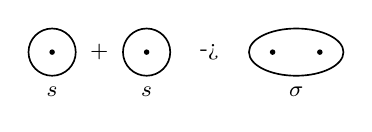
\begin{tikzpicture}
                \footnotesize
                \draw [semithick]
                    (0,0) circle (3mm)
                    (1.2,0) circle (3mm)
                    (3.1,0) ellipse (6mm and 3mm)
                ;

                \fill
                    (0,0) circle (1pt)
                    (1.2,0) circle (1pt)
                    (2.8,0) circle (1pt)
                    (3.4,0) circle (1pt)
                ;
                \node at (0.6,0) {$+$};
                \node at (2,0) {\ce{->}};

                \node at (0,-0.5) {$s$};
                \node at (1.2,-0.5) {$s$};
                \node at (3.1,-0.5) {$\sigma$};
            \end{tikzpicture}
            \caption{Sigma ($\sigma$) bond.}
            \label{fig:sigmaPiDeltaa}
        \end{subfigure}
        \begin{subfigure}[b]{0.3\linewidth}
            \centering
            \begin{tikzpicture}
                \footnotesize
                \filldraw [semithick,fill=grx]
                    (0,0.3) ellipse (3mm and 2mm)
                    (1.2,0.3) ellipse (3mm and 2mm)
                ;
                \draw [semithick]
                    (0,-0.3) ellipse (3mm and 2mm)
                    (1.2,-0.3) ellipse (3mm and 2mm)
                ;
                \draw [semithick,fill=grx] (2.6,0.05)
                    to[out=0,in=180,out looseness=0.5] (3.1,0.12)
                    to[out=0,in=180,in looseness=0.5] (3.6,0.05)
                    to[out=0,in=-90] (3.7,0.15)
                    to[out=90,in=0,out looseness=0.7,in looseness=0.8] (3.1,0.43)
                    to[out=180,in=90,out looseness=0.8,in looseness=0.7] (2.5,0.15)
                    to[out=-90,in=180] cycle
                ;
                \begin{scope}[yscale=-1]
                    \draw [semithick] (2.6,0.05)
                        to[out=0,in=180,out looseness=0.5] (3.1,0.12)
                        to[out=0,in=180,in looseness=0.5] (3.6,0.05)
                        to[out=0,in=-90] (3.7,0.15)
                        to[out=90,in=0,out looseness=0.7,in looseness=0.8] (3.1,0.43)
                        to[out=180,in=90,out looseness=0.8,in looseness=0.7] (2.5,0.15)
                        to[out=-90,in=180] cycle
                    ;
                \end{scope}

                \fill
                    (0,0) circle (1pt)
                    (1.2,0) circle (1pt)
                    (2.8,0) circle (1pt)
                    (3.4,0) circle (1pt)
                ;
                \node at (0.6,0) {$+$};
                \node at (2,0) {\ce{->}};

                \node at (0,-0.7) {$p$};
                \node at (1.2,-0.7) {$p$};
                \node at (3.1,-0.7) {$\pi$};
            \end{tikzpicture}
            \caption{Pi ($\pi$) bond.}
            \label{fig:sigmaPiDeltab}
        \end{subfigure}
        \begin{subfigure}[b]{0.3\linewidth}
            \centering
            \begin{tikzpicture}
                \footnotesize
                \draw [semithick]
                    (0.08,0.01) ellipse (3mm and 2mm)
                    (1.28,0.01) ellipse (3mm and 2mm)
                ;
                \filldraw [semithick,fill=grx]
                    (0,0.3) ellipse (3mm and 2mm)
                    (1.2,0.3) ellipse (3mm and 2mm)
                    (0,-0.3) ellipse (3mm and 2mm)
                    (1.2,-0.3) ellipse (3mm and 2mm)
                ;
                \filldraw [semithick,fill=white]
                    (-0.08,-0.01) ellipse (3mm and 2mm)
                    (1.12,-0.01) ellipse (3mm and 2mm)
                ;
                \draw [semithick]
                    (3.18,0.01) ellipse (6mm and 2mm)
                ;
                \draw [semithick,fill=grx] (2.6,0.05)
                    to[out=0,in=180,out looseness=0.5] (3.1,0.12)
                    to[out=0,in=180,in looseness=0.5] (3.6,0.05)
                    to[out=0,in=-90] (3.7,0.15)
                    to[out=90,in=0,out looseness=0.7,in looseness=0.8] (3.1,0.43)
                    to[out=180,in=90,out looseness=0.8,in looseness=0.7] (2.5,0.15)
                    to[out=-90,in=180] cycle
                ;
                \begin{scope}[yscale=-1]
                    \draw [semithick,fill=grx] (2.6,0.05)
                        to[out=0,in=180,out looseness=0.5] (3.1,0.12)
                        to[out=0,in=180,in looseness=0.5] (3.6,0.05)
                        to[out=0,in=-90] (3.7,0.15)
                        to[out=90,in=0,out looseness=0.7,in looseness=0.8] (3.1,0.43)
                        to[out=180,in=90,out looseness=0.8,in looseness=0.7] (2.5,0.15)
                        to[out=-90,in=180] cycle
                    ;
                \end{scope}
                \filldraw [semithick,fill=white]
                    (3.02,-0.01) ellipse (6mm and 2mm)
                ;

                \fill
                    (0,0) circle (1pt)
                    (1.2,0) circle (1pt)
                    (2.8,0) circle (1pt)
                    (3.4,0) circle (1pt)
                ;
                \node at (0.6,0) {$+$};
                \node at (2,0) {\ce{->}};

                \node at (0,-0.7) {$d$};
                \node at (1.2,-0.7) {$d$};
                \node at (3.1,-0.7) {$\delta$};
            \end{tikzpicture}
            \caption{Delta ($\delta$) bond.}
            \label{fig:sigmaPiDeltac}
        \end{subfigure}
        \caption{Examples of bonding interactions.}
        \label{fig:sigmaPiDelta}
    \end{figure}
    \begin{itemize}
        \item No such bonds exist between carbon atoms because two carbon atoms max out at a triple bond.
        \item Quadruple bonds possess one sigma bond, two pi bonds, and one delta ($\delta$) bond.
        \item The delta bond is only possible with metal atoms because these atoms possess energetically accessible $d$ orbitals.
    \end{itemize}
    \item Quintuple bonds between transition metals have been reported, but scientists have not yet reached a consensus on to what extent these exist.
    \begin{figure}[h!]
        \centering
        \footnotesize
        \chemfig[atom sep=2em,fixed length=true,bond offset=3pt,cram width=3pt]{H-[:-25,,,,dash pattern=on 2pt off 2pt]B(<[:-155]H)(-[7]H?)-[1]H-[7]B?(-[:25,,,,dash pattern=on 2pt off 2pt]H)<[:-25]H}
        \hspace{5em}
        \chemfig[atom sep=2em,fixed length=true,bond offset=3pt,cram width=3pt]{H_3C-[:-25,,,,dash pattern=on 2pt off 2pt]Al(<[:-155]H_3C)(-[7]\chembelow{C}{\hspace{4pt}H_3}?)-[1]\chemabove{C}{\hspace{4pt}H_3}-[7]Al?(-[:25,,,,dash pattern=on 2pt off 2pt]CH_3)<[:-25]CH_3}
        \caption{Inorganic compounds containing bridging hydrogens and alkyl groups.}
        \label{fig:bridgingH-CH3}
    \end{figure}
    \item Hydrogen atoms and alkyl groups can act as bridges in inorganic chemistry, excessively disobeying the octet rule (see Figure \ref{fig:bridgingH-CH3}).
    \item \textbf{Coordination number}: The number of other atoms, molecules, or ions to which an atom is bonded.
    \item "Numerous inorganic compounds have central atoms with coordination numbers of five, six, seven, and higher" \parencite[2]{bib:MiesslerFischerTarr}.
    \begin{itemize}
        \item The most common coordination geometry for transition metals is octahedral.
    \end{itemize}
    \item 4-coordinate carbon is almost always tetrahedral. 4-coordinate metals and nonmetals can be either tetrahedral or square planar.
    \item \textbf{Coordination complex}: A compound with a metal as the central atom or ion and some number of \textbf{ligands} bonded to it.
    \item \textbf{Ligand}: An anion or neutral molecule bonded to a central atom (frequently through \ce{N}, \ce{O}, or \ce{S}).
    \item \textbf{Organometallic complex}: A coordination complex where carbon (potentially bonded to other things) is one of the ligands.
    \begin{figure}[h!]
        \centering
        \footnotesize
        \chemfig[atom sep=5em]{P?[1]-[:53]P(-[6]P?[1]?[3])-[:-53]P?[3]?[1,1,{dash pattern=on 2pt off 2pt}]}
        \caption{Tetrahedral geometry without a central atom.}
        \label{fig:tetrahedralNoCentral}
    \end{figure}
    \item There are multiple kinds of tetrahedral structures. There is the standard arrangement seen in molecules such as methane, but there is also a form that lacks a central atom, as in elemental phosphorous \ce{P4} (see Figure \ref{fig:tetrahedralNoCentral}).
    \begin{itemize}
        \item Other atoms such as boron and carbon also form units that surround a central cavity (e.g., icosahedral \ce{B12} and buckyballs \ce{C60}).
    \end{itemize}
    \item Aromatic rings can bond to metals using all of their pi orbitals. This results in a metal suspended above the ring's center.
    \item \textbf{Cluster compound}: A compound where "a carbon atom is at the center of a polyhedron of metal atoms" \parencite[3]{bib:MiesslerFischerTarr}.
    \begin{itemize}
        \item There exist examples of carbon surrounded by five, six, or more metal atoms\footnote{This provides a challenge to theoretical inorganic chemists.}.
    \end{itemize}
    \item Many new forms of elemental carbon have been discovered since the mid-1980s, notably including fullerenes (such as buckminsterfullerene, or buckyballs), carbon nanotubes, graphene, and polyyne wires.
    \item \textcite{bib:MiesslerFischerTarr} give a brief history of inorganic chemistry for context.
    \begin{itemize}
        \item Be aware of \textbf{crystal field theory} and \textbf{ligand field theory}.
    \end{itemize}
\end{itemize}
\newpage



\section{Chapter 2: Atomic Structure}
\emph{From \textcite{bib:MiesslerFischerTarr}.}
\subsection{Problems}
\begin{enumerate}[label={\textbf{2.\arabic*}}]
    \setcounter{enumi}{7}
    \item \marginnote{9/13:}The details of several steps in the particle-in-a-box model in this chapter have been omitted. Work out the details of the following steps:
    \begin{enumerate}[label={\textbf{\alph*.}}]
        \item Show that if $\Psi=A\sin rx+B\cos sx$ ($A$, $B$, $r$, and $s$ are constants) is a solution to the wave equation for the one-dimensional box, then
        \begin{equation*}
            r = s = \sqrt{2mE}\left( \frac{2\pi}{h} \right)
        \end{equation*}
        \begin{proof}[Solution]
            \allowdisplaybreaks
            \begin{align*}
                \frac{-h^2}{8\pi^2m}\cdot\pdv[2]{\Psi(x)}{x} &= E\Psi(x)\\
                \frac{-h^2}{8\pi^2m}\cdot\pdv[2]{x}\left( A\sin rx+B\cos sx \right) &= E(A\sin rx+B\cos sx)\\
                \frac{-h^2}{8\pi^2m}\cdot\pdv{x}\left( Ar\cos rx-Bs\sin sx \right) &= E(A\sin rx+B\cos sx)\\
                \frac{-h^2}{8\pi^2m}\cdot\left( -Ar^2\sin rx-Bs^2\cos sx \right) &= E(A\sin rx+B\cos sx)\\
                \frac{Ar^2h^2}{8\pi^2m}\sin rx+\frac{Bs^2h^2}{8\pi^2m}\cos sx &= AE\sin rx+BE\cos sx\\
                0 &= \left( \frac{Ar^2h^2}{8\pi^2m}-AE \right)\sin rx+\left( \frac{Bs^2h^2}{8\pi^2m}-BE \right)\cos sx
                \intertext{Choose $x=0$.}
                &= \frac{Bs^2h^2}{8\pi^2m}-BE\\
                E &= \frac{s^2h^2}{8\pi^2m}\\
                \frac{8\pi^2mE}{h^2} &= s^2\\
                s &= \sqrt{\frac{8\pi^2mE}{h^2}}\\
                \Aboxed{s &= \sqrt{2mE}\frac{2\pi}{h}}
                \intertext{With this result \dots}
                0 &= \left( \frac{Ar^2h^2}{8\pi^2m}-AE \right)\sin rx+\left( \frac{Bs^2h^2}{8\pi^2m}-BE \right)\cos sx\\
                &= \left( \frac{Ar^2h^2}{8\pi^2m}-AE \right)\sin rx+\left( B\left( \frac{s^2h^2}{8\pi^2m} \right)-BE \right)\cos sx\\
                &= \left( \frac{Ar^2h^2}{8\pi^2m}-AE \right)\sin rx+\left( BE-BE \right)\cos sx\\
                &= \left( \frac{Ar^2h^2}{8\pi^2m}-AE \right)\sin rx\\
                \intertext{Choose $x=\frac{\pi}{2r}$.}
                &= \frac{Ar^2h^2}{8\pi^2m}-AE\\
                \Aboxed{r &= \sqrt{2mE}\frac{2\pi}{h}}
            \end{align*}
        \end{proof}
        \setcounter{enumii}{3}
        \item Show that substituting the value of $r$ given in part c into $\Psi=A\sin rx$ and applying the normalizing requirement gives $A=\sqrt{2/a}$.
        \begin{proof}[Solution]
            \begin{align*}
                1 &= \int_\text{all space}\Psi\Psi^*\dd{\tau}\\
                &= \int_0^a \left( A\sin\frac{n\pi x}{a} \right)\left( A\sin\frac{n\pi x}{a} \right)\dd{x}\\
                &= \int_0^a A^2\sin^2\frac{n\pi x}{a}\dd{x}
                \intertext{Use $\sin^2u=\frac{1-\cos2u}{2}$.}
                &= A^2\int_0^a \frac{1-\cos\frac{2n\pi x}{a}}{2}\dd{x}\\
                &= \frac{A^2}{2}\left( \int_0^a \dd{x}-\int_0^a \cos\frac{2n\pi x}{a}\dd{x} \right)\\
                &= \frac{A^2}{2}\left( [x]_0^a-\left[ \frac{a}{2n\pi}\sin\frac{2n\pi x}{a} \right]_0^a \right)\\
                &= \frac{A^2}{2}\left( (a-0)-\left( \frac{a}{2n\pi}\sin 2n\pi-\frac{a}{2n\pi}\sin 0 \right) \right)\\
                &= \frac{A^2}{2}\left( a-\left( \frac{a}{2n\pi}\sin 2n\pi \right) \right)
                \intertext{Since $n$ is an integer, $\sin 2n\pi=0$.}
                &= \frac{aA^2}{2}\\
                \frac{2}{a} &= A^2\\
                \Aboxed{A &= \sqrt{\frac{2}{a}}}
            \end{align*}
        \end{proof}
    \end{enumerate}
\end{enumerate}




\end{document}